\chapter{Implementation}

\section{Tools used}

\subsection*{Sublime Text}

\begin{figure}[h]
    \centering
    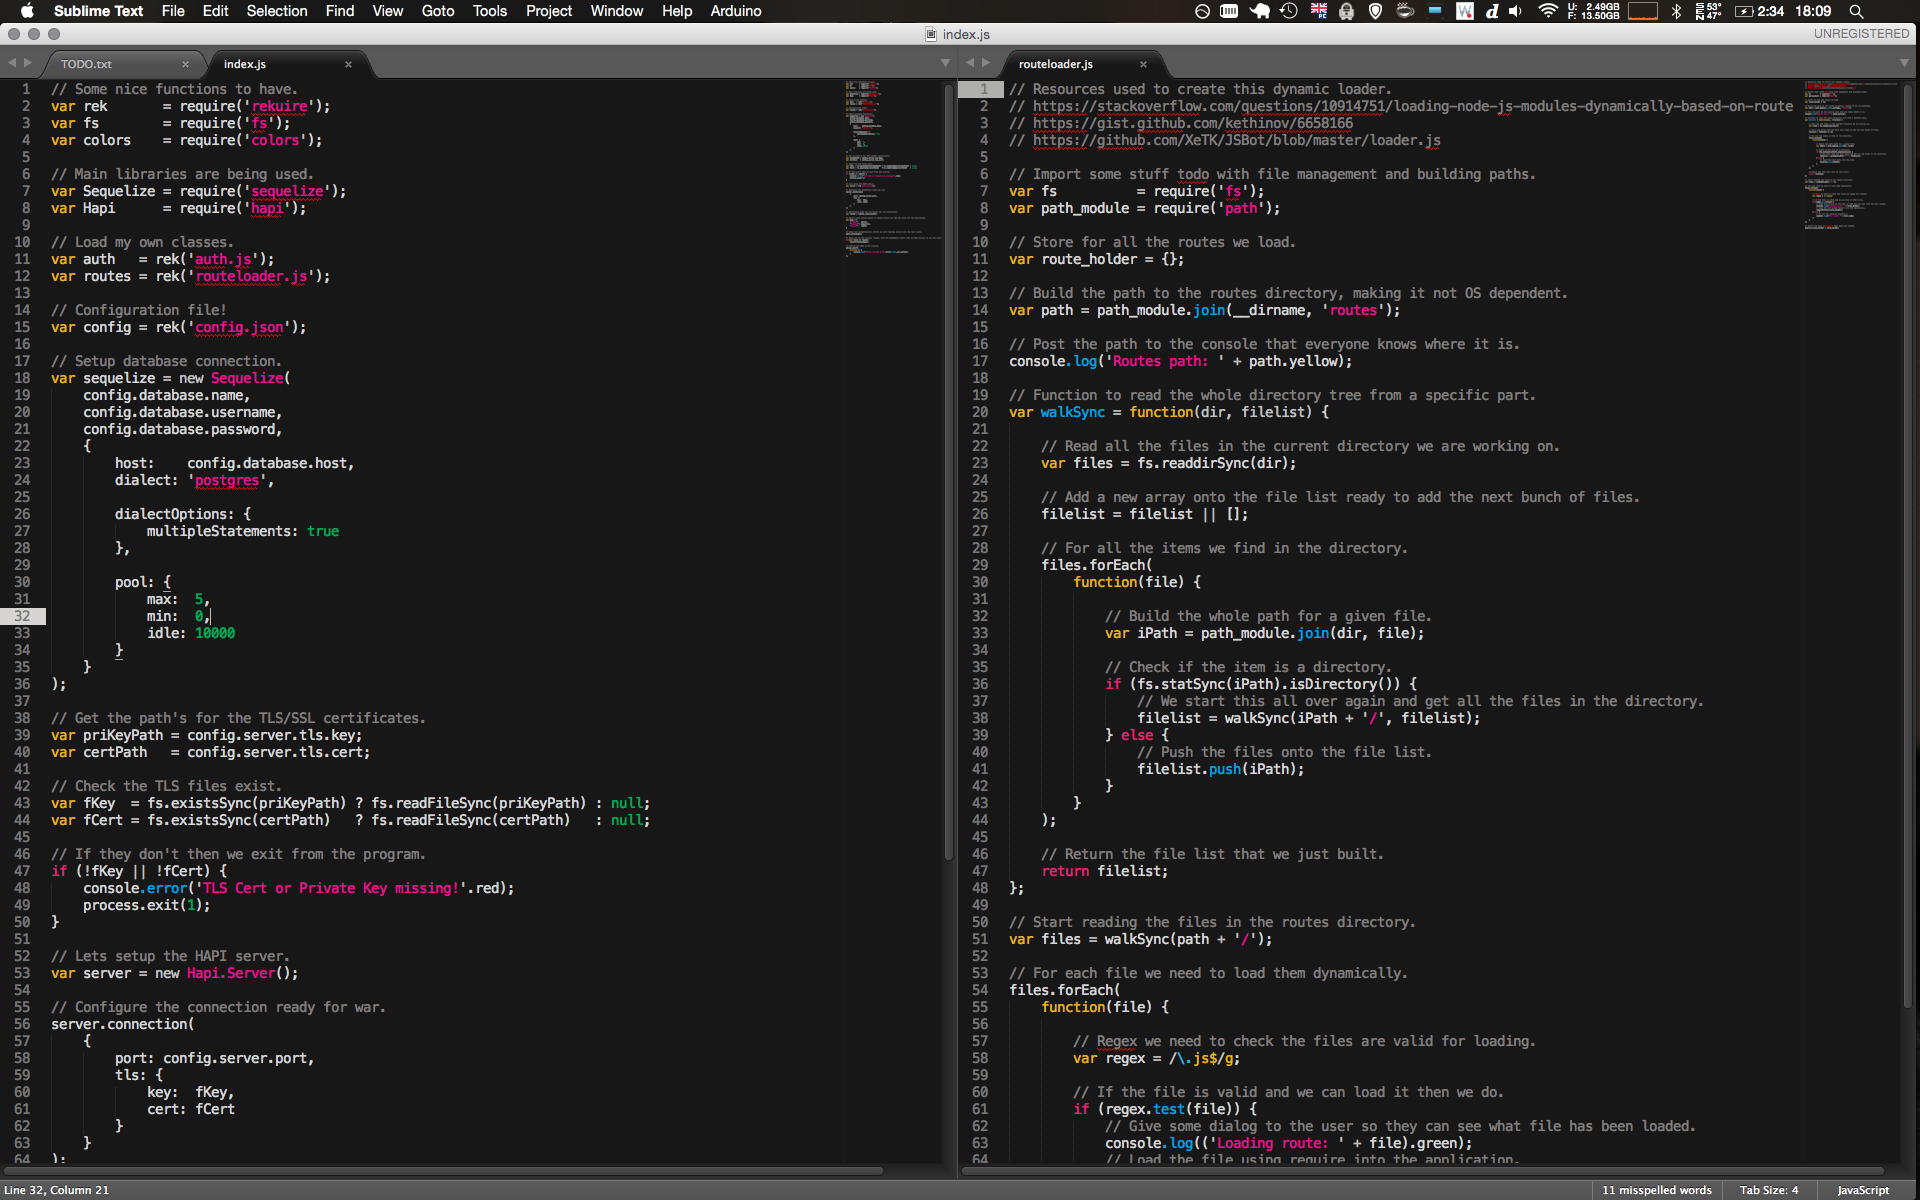
\includegraphics[width=\textwidth]{tools/sublime}
    \caption{Sublime Text 3.0}
    \label{fig:sublime_text_image}
\end{figure} 
\noindent

\subsection*{Android Studio}

\begin{figure}[h]
    \centering
    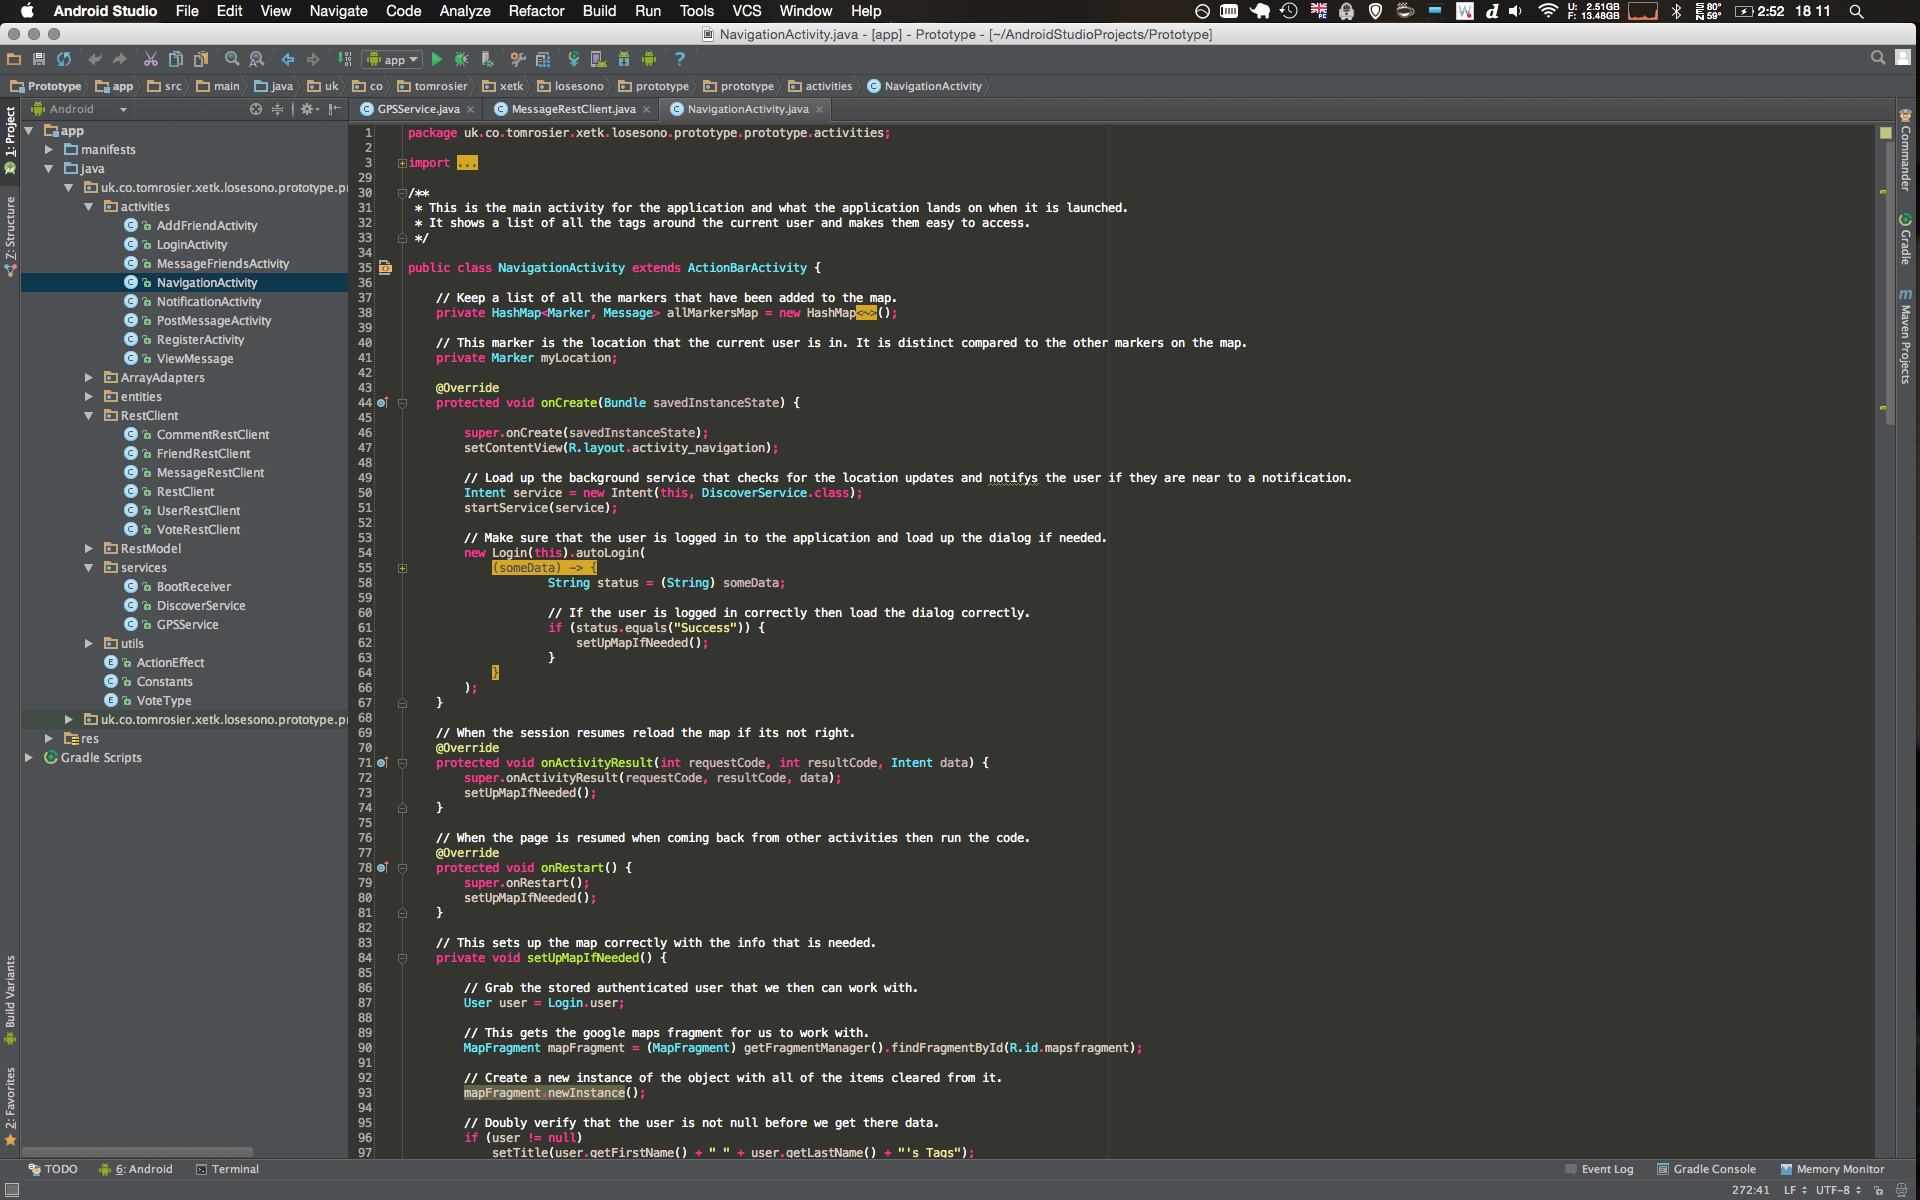
\includegraphics[width=\textwidth]{tools/androidstudio}
    \caption{Android Studio 1.1.0}
    \label{fig:android_studio_image}
\end{figure} 
\noindent

\subsection*{PGAdmin3}

\begin{figure}[h]
    \centering
    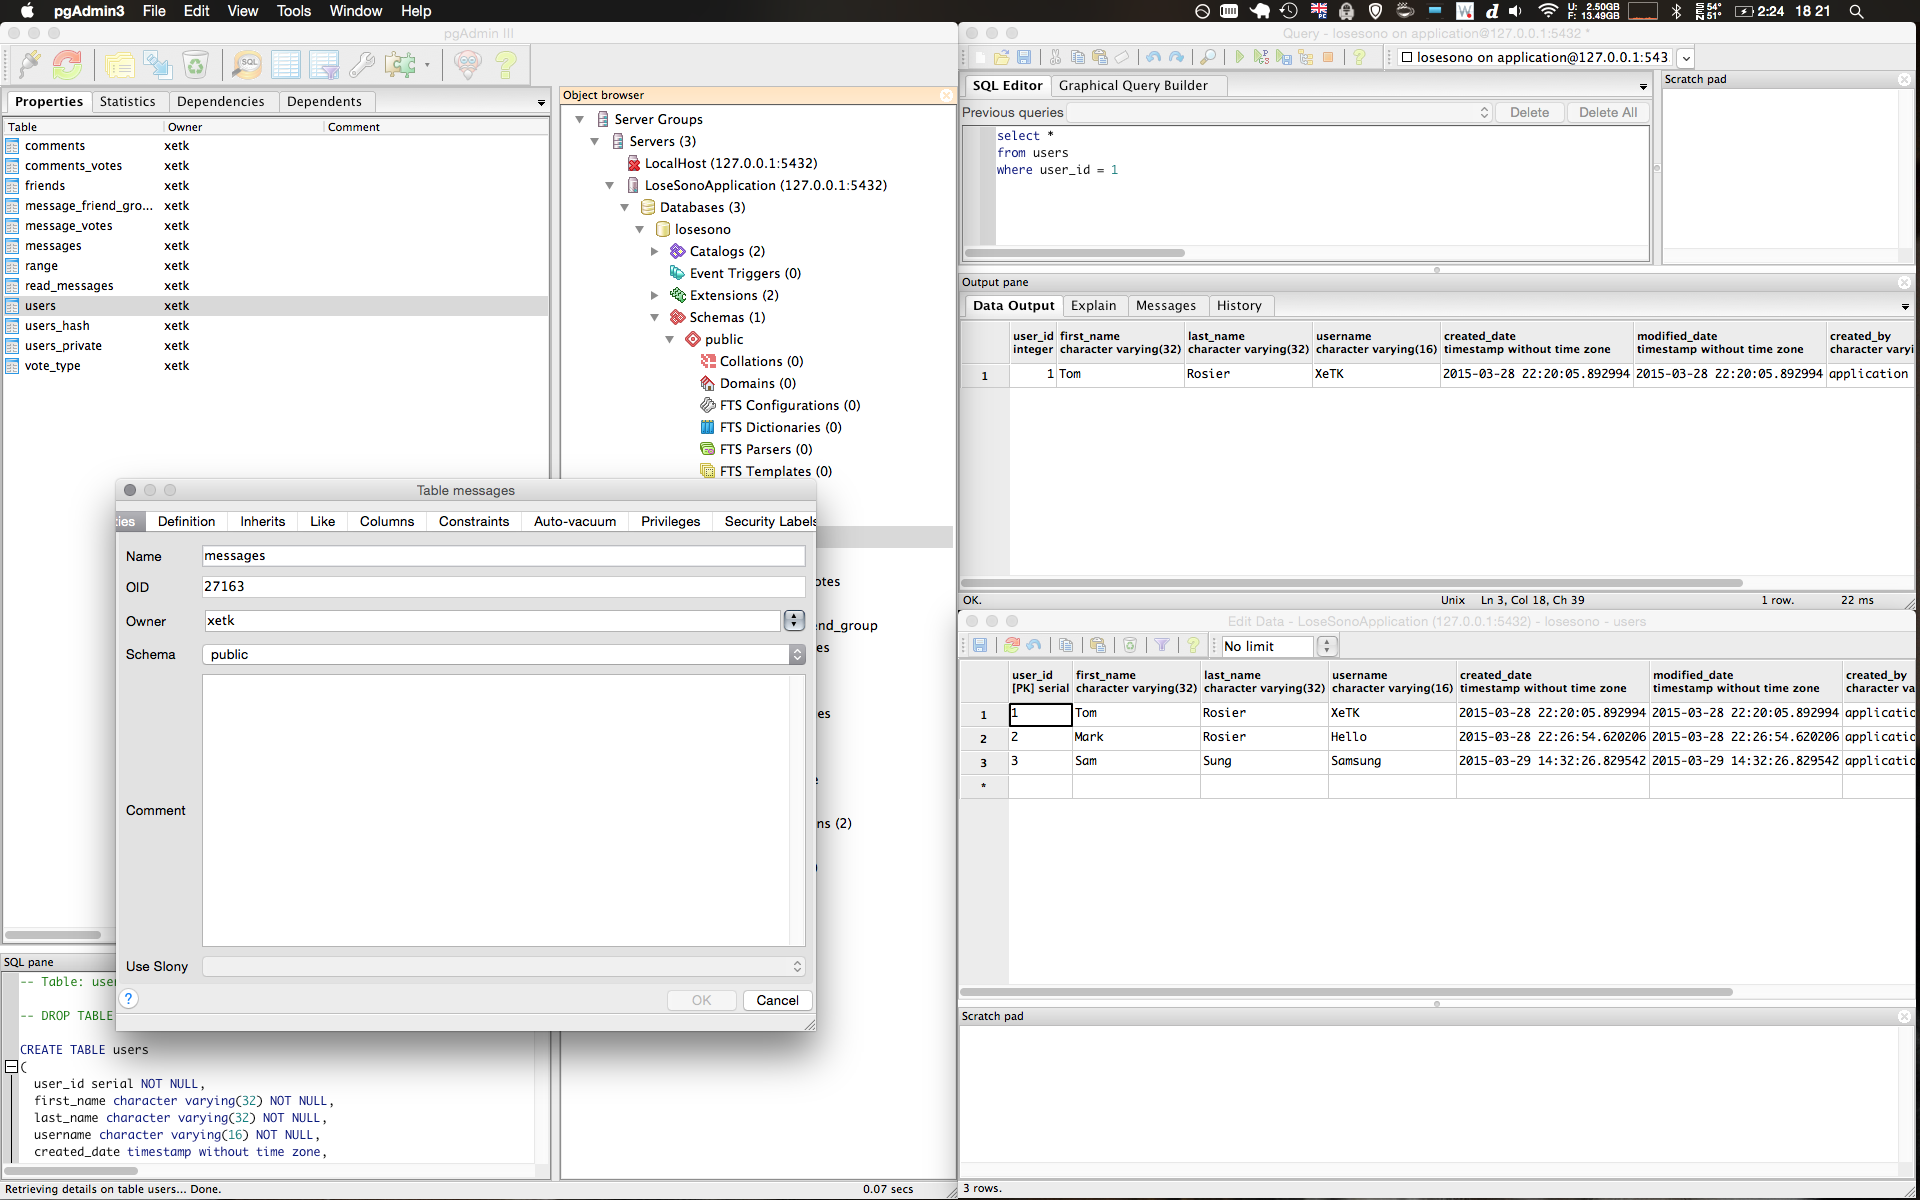
\includegraphics[width=\textwidth]{tools/pgadmin}
    \caption{PGAdmin 1.20.0}
    \label{fig:pg_admin_image}
\end{figure} 
\noindent

\subsection*{Postman}

\begin{figure}[h]
    \centering
    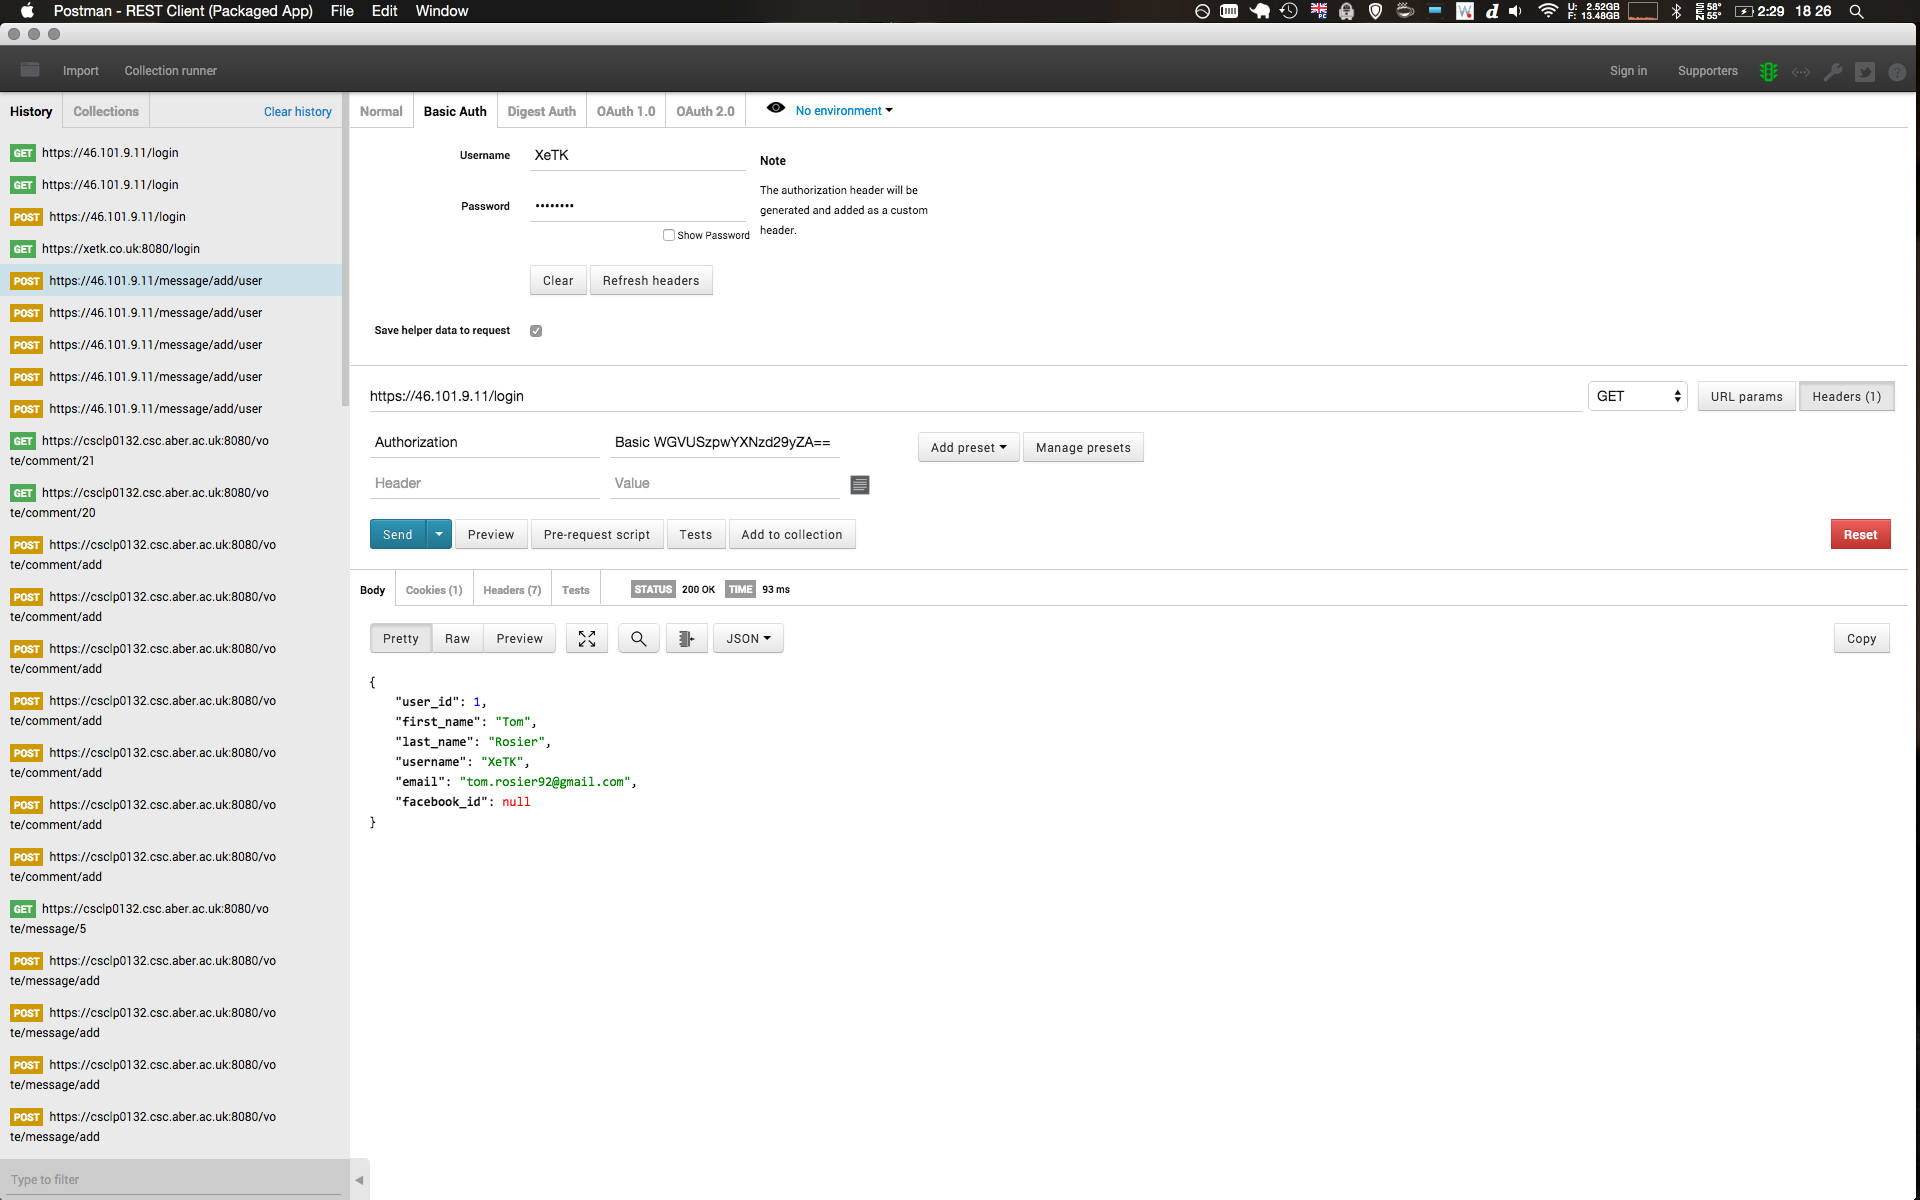
\includegraphics[width=\textwidth]{tools/postman}
    \caption{Postman 2.0.19}
    \label{fig:postman_image}
\end{figure} 
\noindent

\subsection*{Web browsers}

\begin{figure}[h]
    \centering
    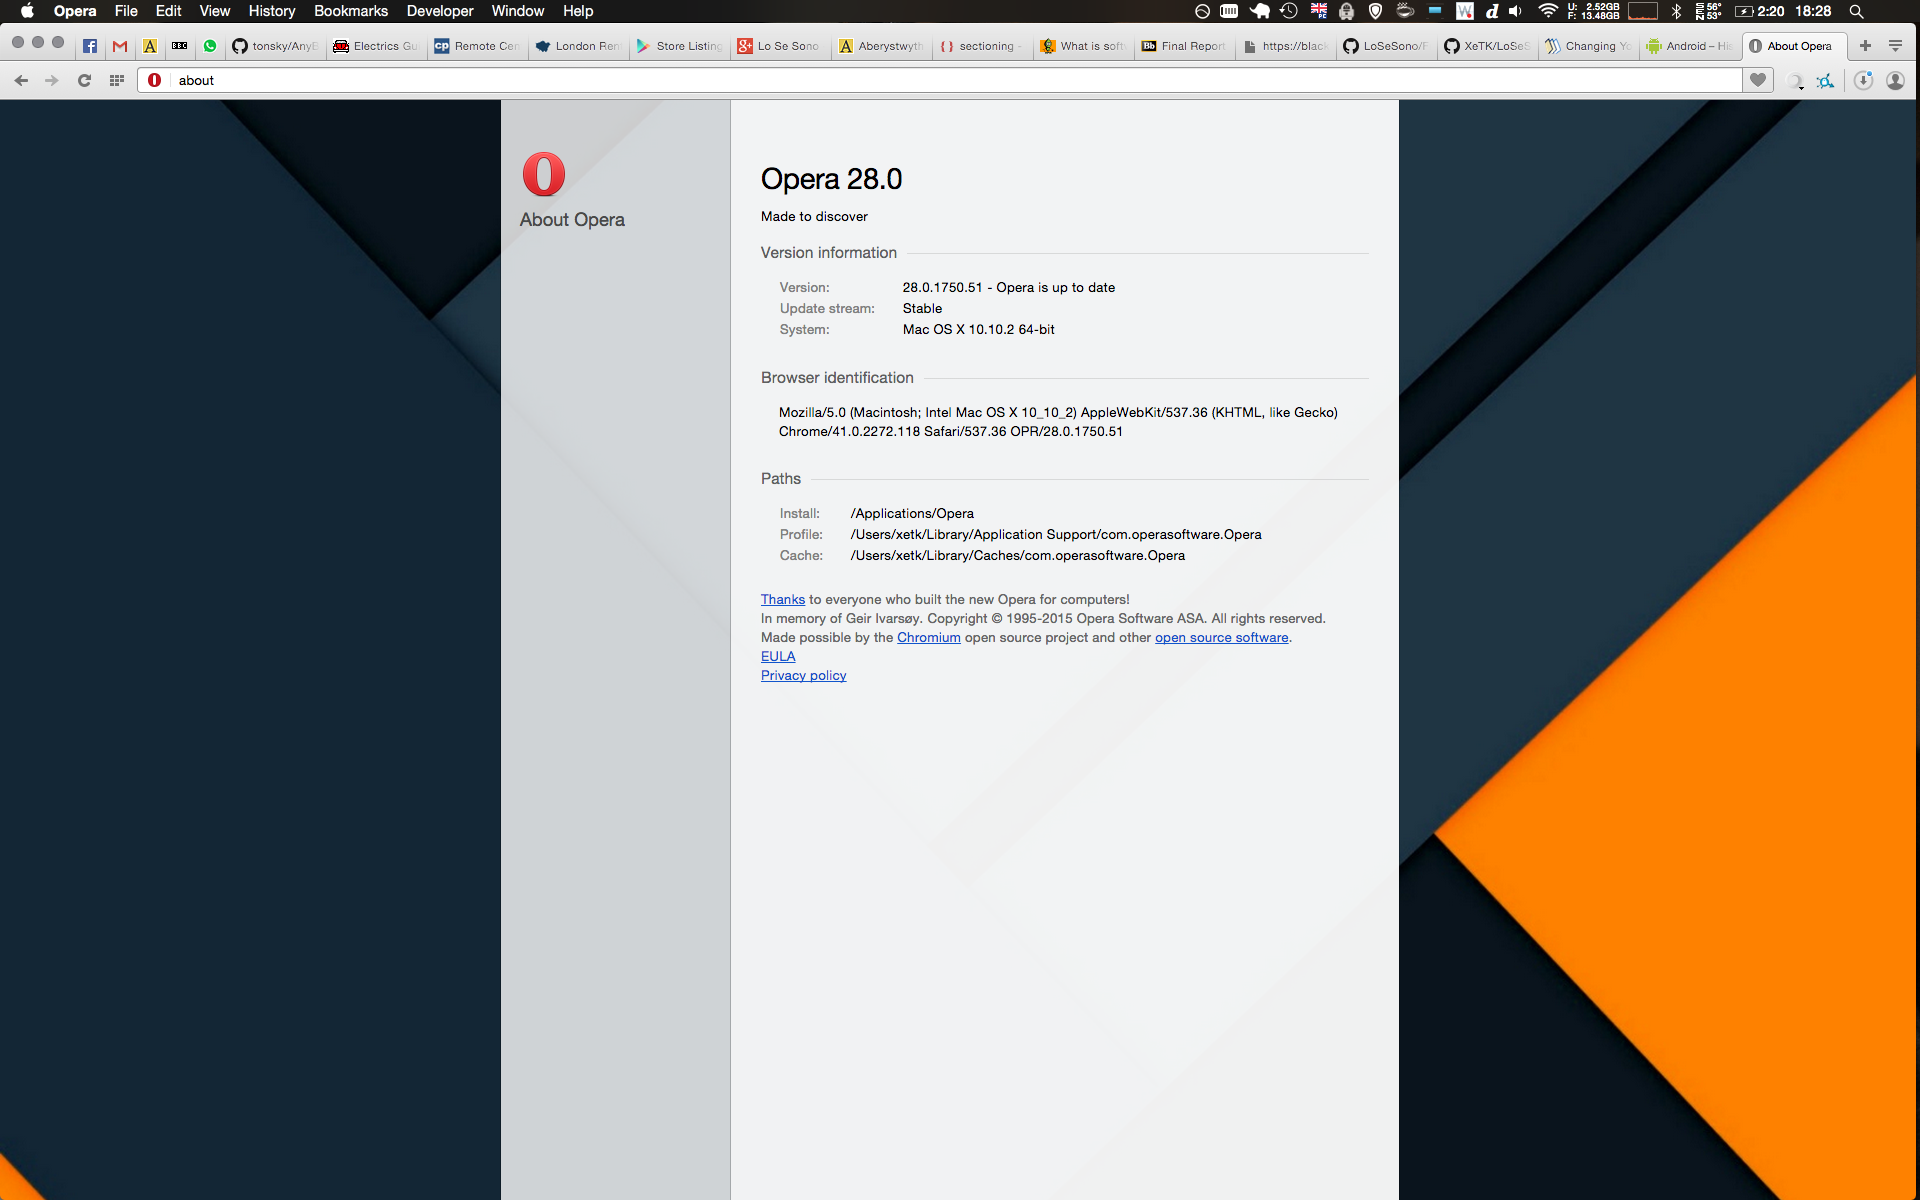
\includegraphics[width=\textwidth]{tools/opera}
    \caption{Opera 28.0}
    \label{fig:opera_image}
\end{figure} 
\noindent

\begin{figure}[h]
    \centering
    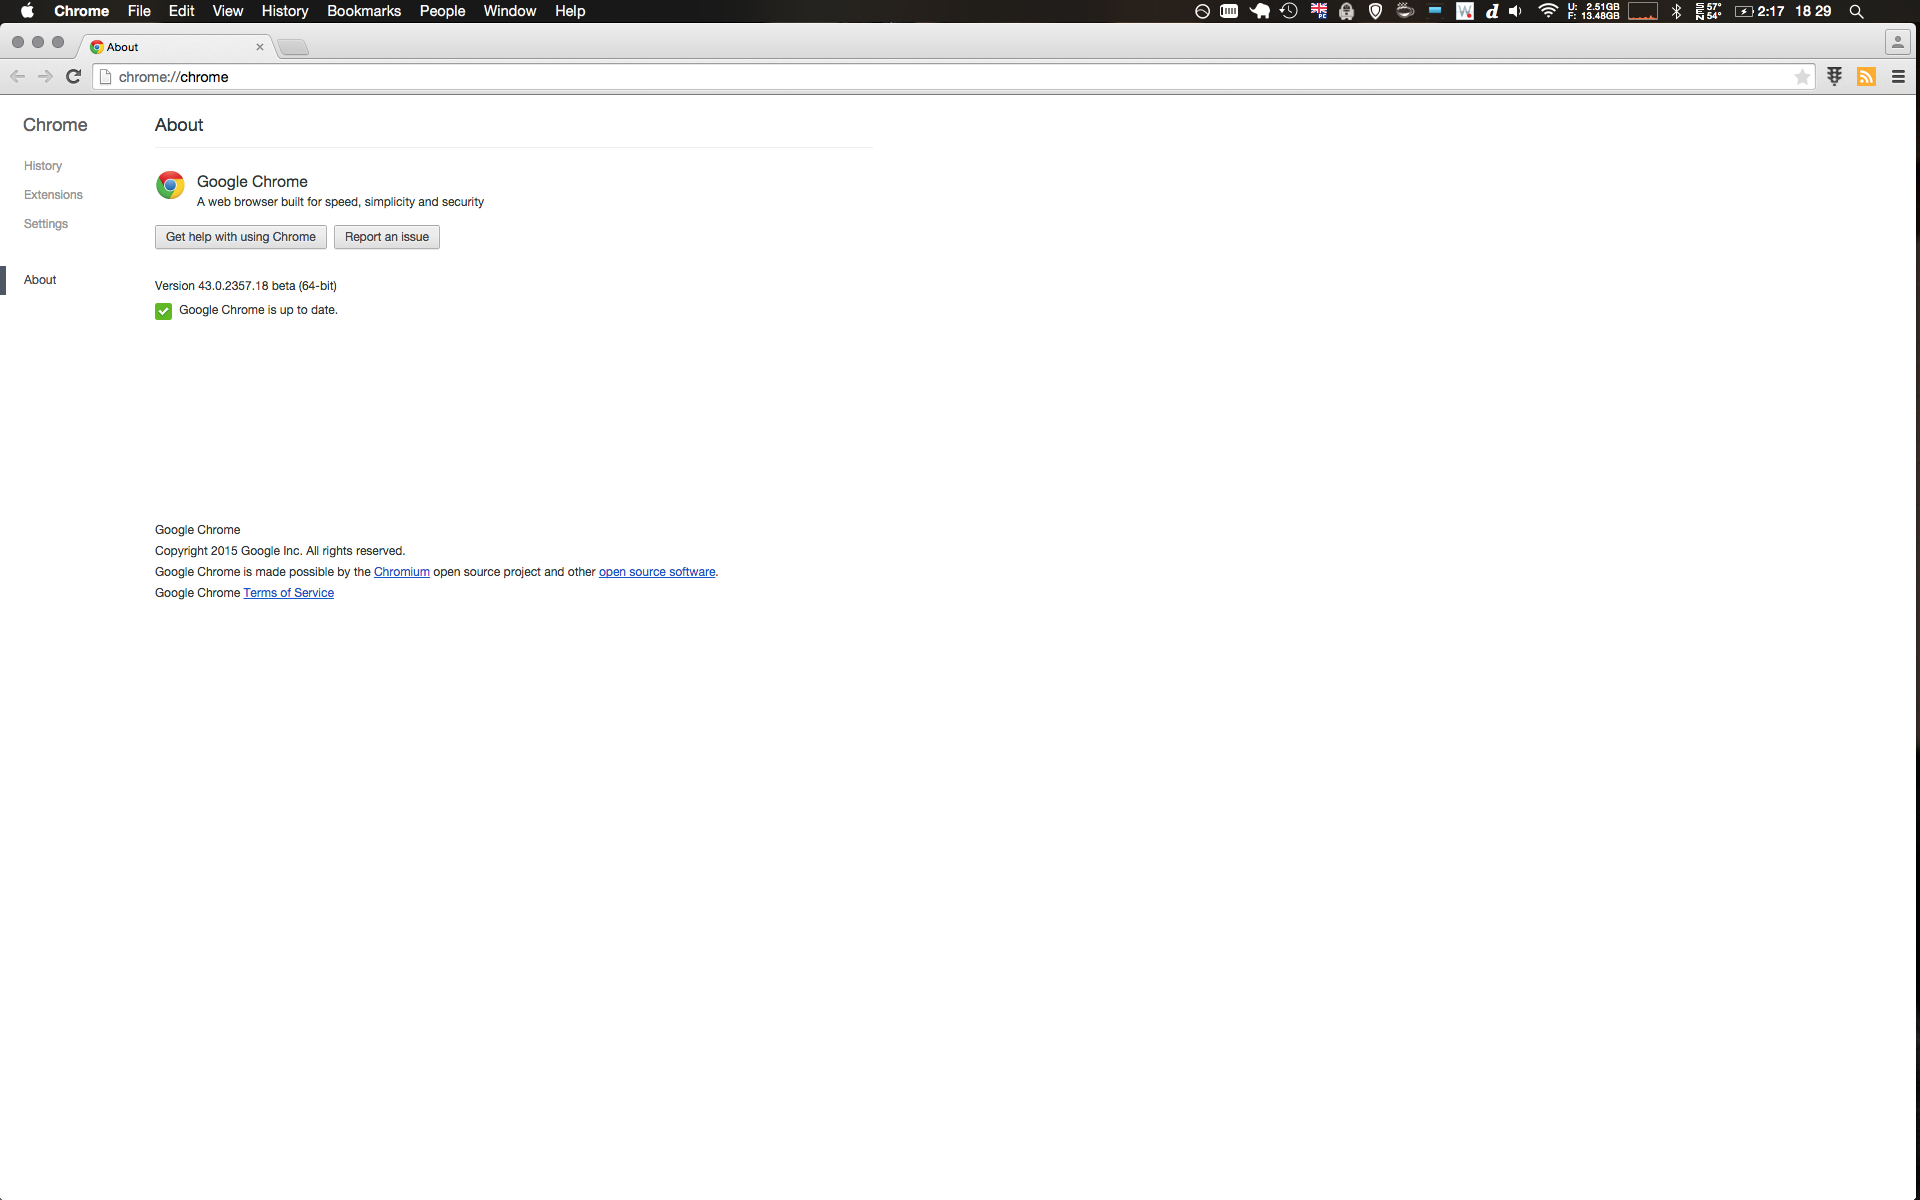
\includegraphics[width=\textwidth]{tools/chrome}
    \caption{Chrome 43.0}
    \label{fig:opera_image}
\end{figure} 
\noindent

\subsection*{Android SDK Tools}

\begin{figure}[h]
    \centering
    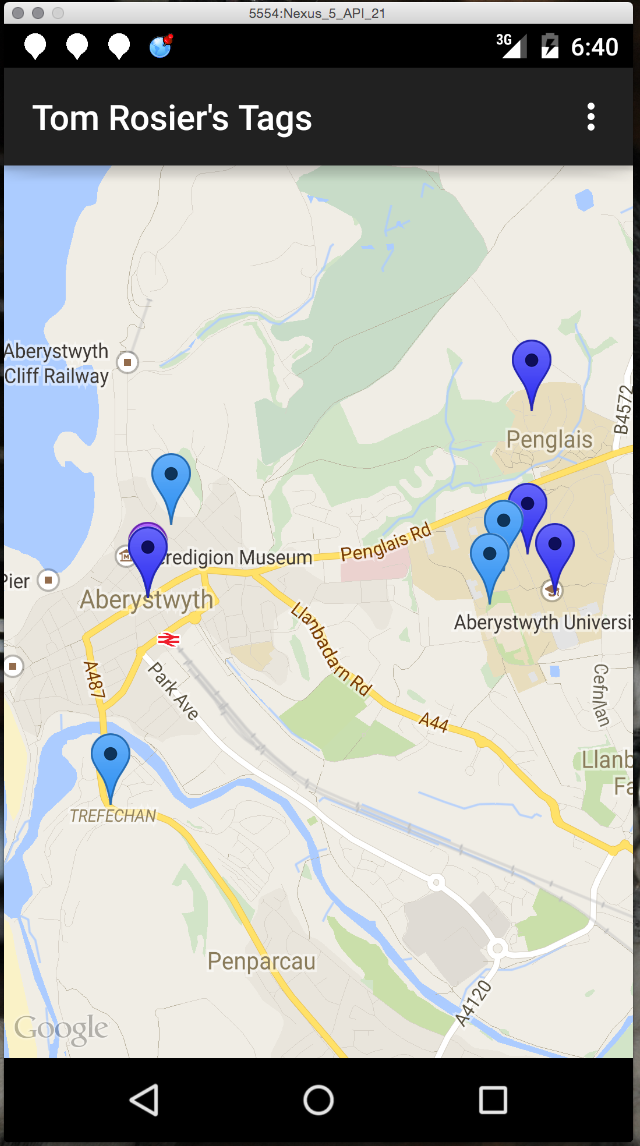
\includegraphics[width=0.5\textwidth]{tools/androidemulator}
    \caption{Android Emulator SDK 22}
    \label{fig:android_emulator}
\end{figure} 
\noindent

\begin{figure}[h]
    \centering
    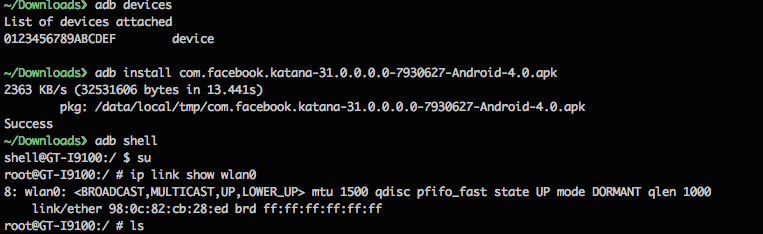
\includegraphics[width=0.75\textwidth]{tools/adb}
    \caption{Android Development Bridge}
    \label{fig:adb_image}
\end{figure} 
\noindent

\begin{figure}[h]
    \centering
    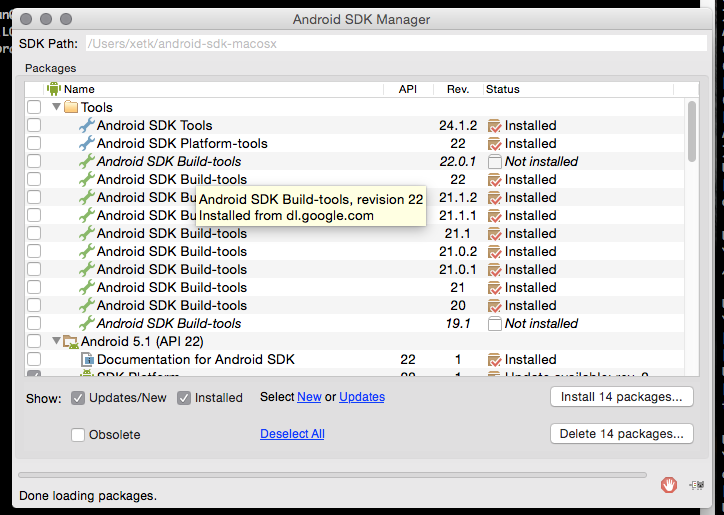
\includegraphics[width=0.75\textwidth]{tools/sdkupdator}
    \caption{Android SDK Updater}
    \label{fig:sdk_updator}
\end{figure} 
\noindent

\subsection*{Git Hub}

\begin{figure}[h]
    \centering
    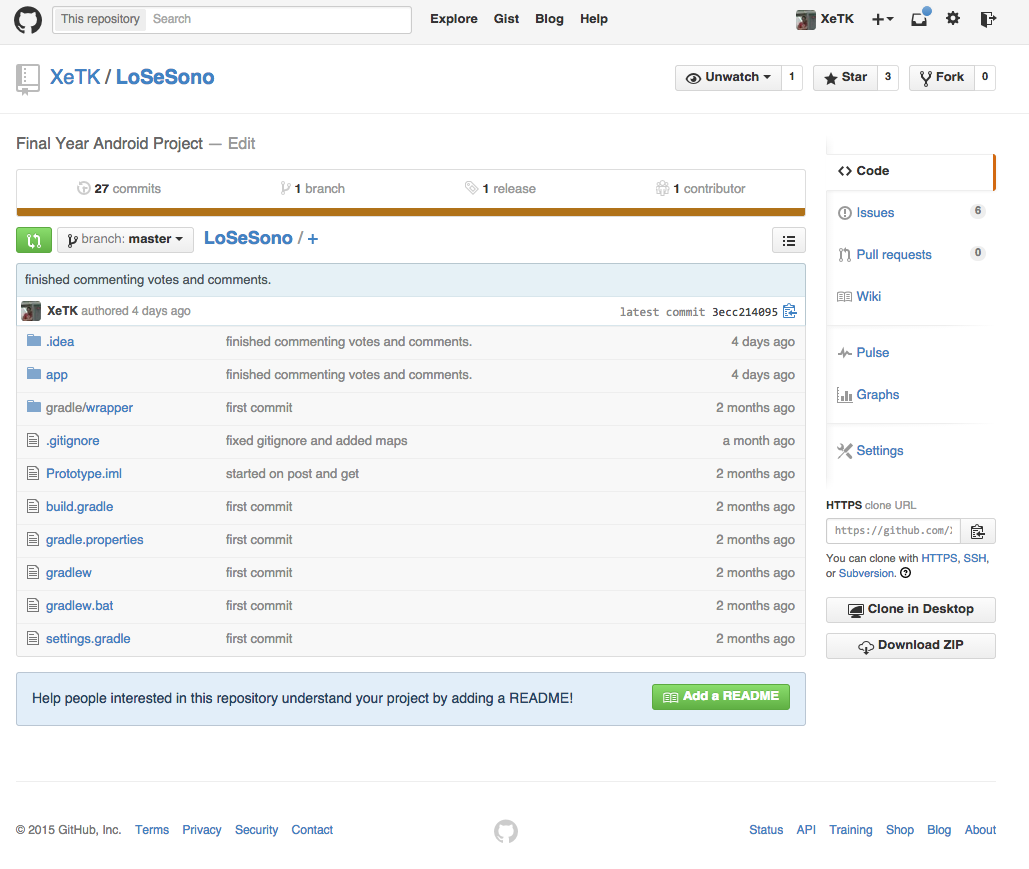
\includegraphics[width=\textwidth]{tools/github}
    \caption{Git Hub git repositories}
    \label{fig:git_hub_repos_image}
\end{figure} 
\noindent

\begin{figure}[h]
    \centering
    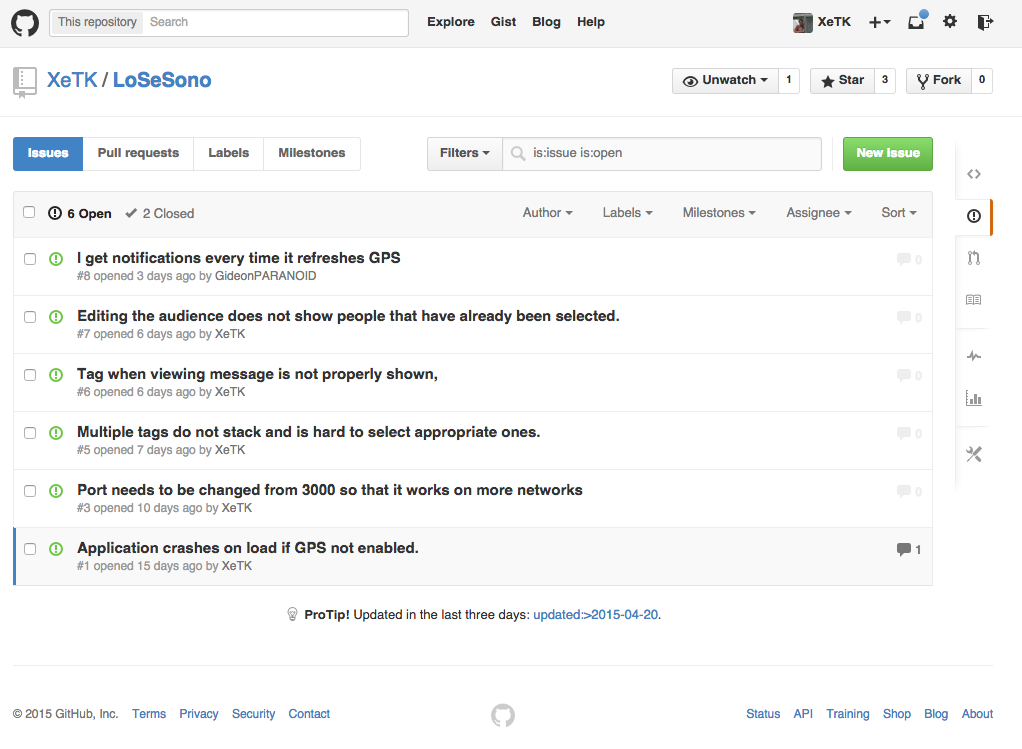
\includegraphics[width=\textwidth]{tools/githubissues}
    \caption{Github issue tracker}
    \label{fig:gh_issue_tracker_image}
\end{figure} 
\noindent

\subsection*{PGSQL command line}

\begin{figure}[h]
    \centering
    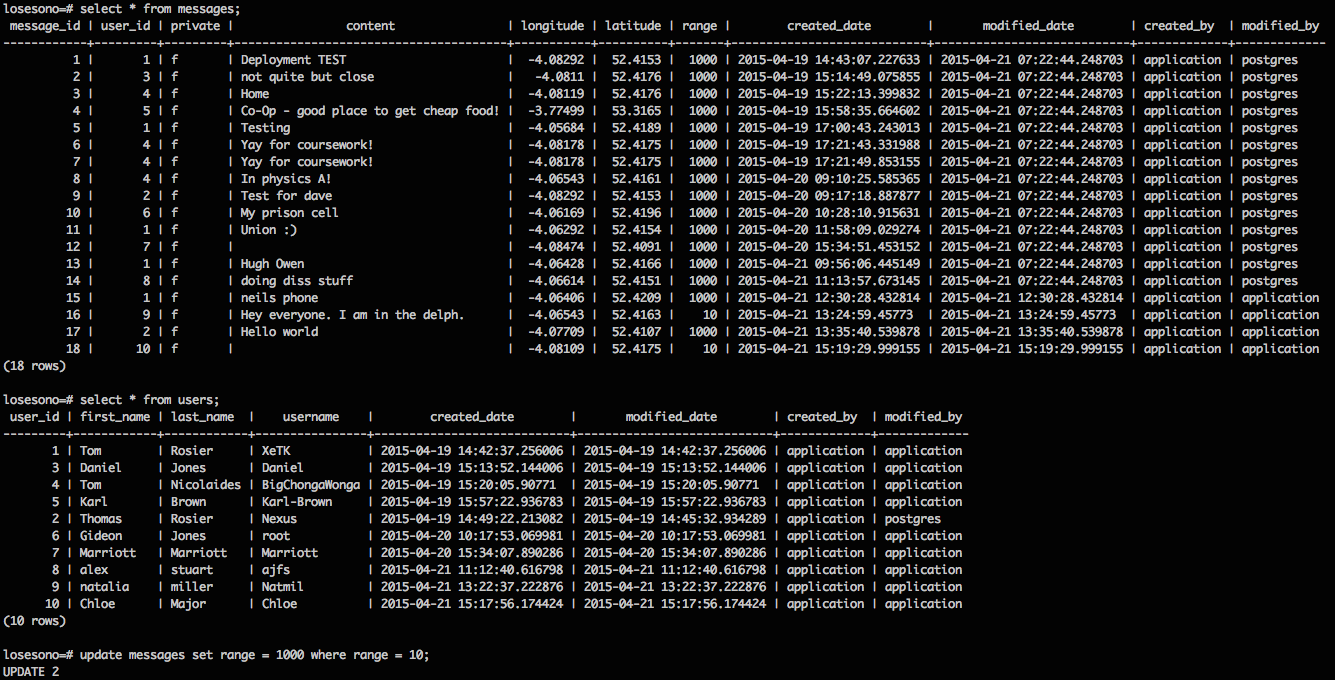
\includegraphics[width=\textwidth]{tools/pgsqlcommandline}
    \caption{PG SQL Command line 9.3.6}
    \label{fig:pg_sql_image}
\end{figure} 
\noindent


\section{Android application}

\subsection{Development Hardware}

\subsection{Environment}

\subsection{Features}


\subsubsection*{Login}

\paragraph*{Implementation}

\paragraph*{Issues}


\subsubsection*{Registration}

\paragraph*{Implementation}

\paragraph*{Issues}


\subsubsection*{Adding Friends}

\paragraph*{Implementation}

\paragraph*{Issues}


\subsubsection*{GPS Location}

\paragraph*{Implementation}

\paragraph*{Issues}


\subsubsection*{Maps}

\paragraph*{Implementation}

\paragraph*{Issues}


\subsubsection*{Posting message}

\paragraph*{Implementation}

\paragraph*{Issues}


\subsubsection*{Retrieving messages}

\paragraph*{Implementation}

\paragraph*{Issues}


\subsubsection*{Retrieving notifications}

\paragraph*{Implementation}

\paragraph*{Issues}


\subsubsection*{Comments}

\paragraph*{Implementation}

\paragraph*{Issues}


\subsubsection*{Votes}

\paragraph*{Implementation}

\paragraph*{Issues}



\section{Server side application}


\subsection{Environment}

\subsubsection{Debian based Linux}

\subsubsection{Postgres Database}

\subsubsection{Node.js environment}

\subsubsection{Digital Ocean Droplet}

% Ram issues


\subsection{Middle tier application}

\subsubsection{Core functionality}

\subsubsection{Rest Interface}

\subsubsection{Database Connector}


\subsection{Database level}

\subsubsection{Tables}

\subsubsection{Functions}


\section{Review of implementation}